%!Tex Root = ../main.tex
% ./Packete.tex
% ./Design.tex
% ./Deklarationen.tex
% ./Vorbereitung.tex
% ./Aufgabe1.tex
% ./Aufgabe2.tex
% ./Aufgabe3.tex
% ./Aufgabe4.tex

\section{Bonus}

\begin{frame}[allowframebreaks]{Bonus}{Vollständige Induktion über natürliche Zahlen\vspace{0.5cm}}
  \begin{itemize}
    \item für \alert{Allbehauptungen}: $\forall n\in\mathbb{N}:\mathcal{E}(n)$ (Eigenschaft $\mathcal{E}$)
    \item die allgemeine Form wird als \alert{Strukturelle Induktion} bezeichnet, \alert{Vollständige Induktion} ist zum Beweis von Aussagen für alle Natürlichen Zahlen
    \begin{itemize}
      \item Menge der \alert{natürlichen Zahlen} $\mathbb{N}$ weißt geignete Struktur auf, da auf ihnen die Nachfolgerbeziehung besteht
    \end{itemize}
    \item man führt Teilbewise für $2$ Fälle: 
    \begin{itemize}
      \item \alert{Basisfall:} ${\mathcal{E}}(0)$, d.h. die natürliche Zahl $0$ hat die Eigenschaft $\epsilon$
      \item \alert{Induktionsfall:} $\forall i\in\mathbb{N} \left(\mathcal{E}(i)\Rightarrow\mathcal{E}(i+1)\right)$, d.h. die Eigenschaft $\epsilon$ überträgt sich von jeder natürlichen Zahl $i$ auf ihren Nachfolger $i + 1$
    \end{itemize}
    \item bei beweisender Allbehauptung für den Induktionsfall wird Implikation: Sei $i\in\mathbb{N}$ beliebig. Zu zeigen: $\epsilon(i)\Rightarrow\epsilon(i+1)$ zerlegt in: Sei $i\in\mathbb{N}$ beliebig. Es gelte: $\epsilon(i)$. Zu zeigen: $\epsilon(i+1)$
    \item Diese Darstellung des Induktionsfalls legt seine Zerlegung in die üblichen drei Bestandteile \alert{Induktionsannahme}, \alert{Induktionsbehauptung}, \alert{Induktionsschritt} nahe:
  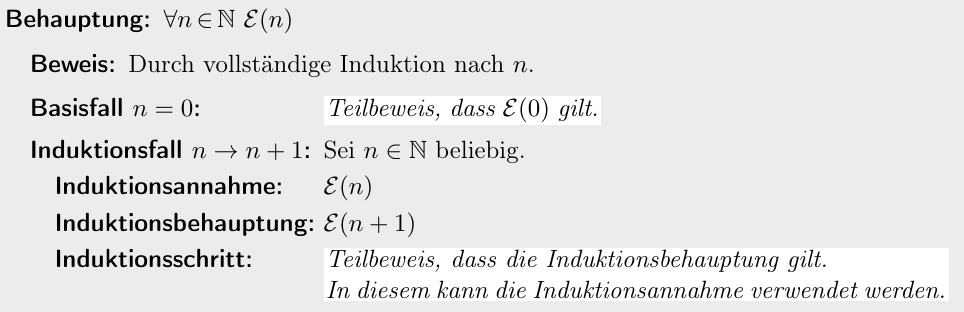
\includegraphics[width=\linewidth]{./figures/vollstaendige_induktion.png}
  \end{itemize}
  \begin{itemize}
    \item Induktionsfall beweist Allbehauptung mit darin enthaltener Implikationsbehauptung 
    \item Wenn für Eigenschaft $\epsilon$ Basisfall und Induktionsfall bewiesen sind, gilt, dass jede natürliche Zahl die Eigenschaft $\epsilon$ hat, denn:
    \begin{enumerate}
      \setcounter{enumi}{-1}
      \item Wegen des Basisfalls gilt $\epsilon(0)$.
      \item Mit $\epsilon(0)$ gilt wegen des Induktionsfalls auch $\epsilon(1)$.
      \item Mit $\epsilon(1)$ gilt wegen des Induktionsfalls auch $\epsilon(2)$.
      \item Mit $\epsilon(2)$ gilt wegen des Induktionsfalls auch $\epsilon(3)$.
      \item $\ldots$
    \end{enumerate}
    \item asdf
  \end{itemize}
  \begin{example}{Vollstständige Induktion}
    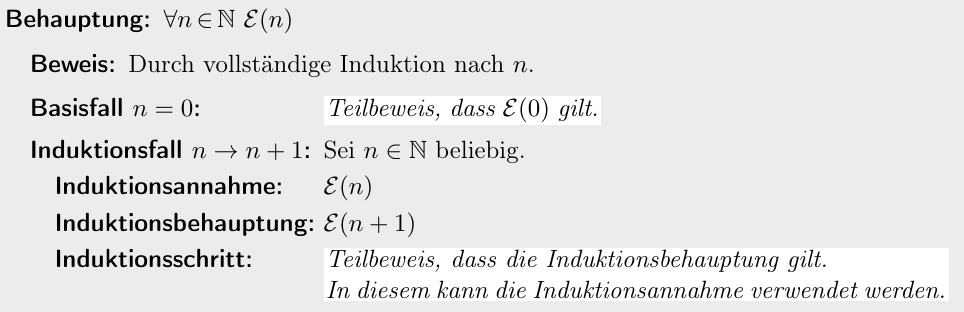
\includegraphics[width=\textwidth]{./figures/vollstaendige_induktion.png}
  \end{example}
\end{frame}

\begin{frame}{Bonus}{Regel von L'Hopital}
  \begin{itemize}
    \item asdf
  \end{itemize}
\end{frame}
